\documentclass{mcmthesis}
\mcmsetup{CTeX = false,   % 使用 CTeX 套装时,设置为 true
        tcn =89324 , problem = B, 
        sheet = true, titleinsheet = true, keywordsinsheet = true, 
        titlepage = false, abstract = true}
\usepackage{palatino}
\usepackage{lipsum}
\usepackage{diagbox}
\usepackage{color}
\usepackage{hyperref}
\hypersetup{colorlinks=true, linkcolor=black}
\title{Open Offices Mathematically}
\author{}
\date{\today}
\begin{document}
\begin{abstract}
In this paper, we examine the trends of various languages' number and distribution over the future fifty years through mathematically analyzing the historic evolution of various languages. Divide the total language speakers into two groups--- native speakers and second-language speakers, we use age-dependent population system and neutral network respectively to calculate the future number of total speakers. Then we model the language distribution evolution trend through analyzing the possible extension of various languages. The conclusion can be drawn that the scope of English will increase greatly while Bangladesh region will shrink. Other language such as Japanese and Russian will maintain steady. After fifty years, the total speakers of Punjabi will exceed that of French and rank tenth for the higher birth rate of Pakistan.\\
\indent For the problem of locating new offices, the location optimization model is constructed to make the company a huge benefit as well as achieving internationalization. We formulate the selection process with the help of the prediction of future language distribution. To demonstrate how our model works, we compare the results with the overseas branch of Microsoft Corporation and McKinsey \& Company. By calculating the average score of choosing locations, we conclude that it is more reasonable to choose five locations for the sake of saving the company resources. 
\begin{keywords}
Language Distribution; Number of Language Speaker; Location of the Offices; BP Neutral Network; 0-1 Multi-objective Programming; Genetic Algorithm. 
\end{keywords}
\end{abstract}
\maketitle
\tableofcontents
\newpage
\section{Introduction}
As the basis of communication and cooperation, language plays an important role in our daily life. Thus, the studies on the language distribution have been gaining more and more attention. M.A.F Gomes (2001) found the relationship between the distribution of languages and geometrical aspects. Also, the predictions of the future top five world languages have been made by Kirsten Winkler (2012).\\
\indent However, since multiple factors affecting the language distribution such as the official languages, education policies, immigration between countries, increased culture communication and so on, few works have been down to reasonably picture the future language distribution. Thus, we intended to further the study by taking more factors into consideration and calculate numbers of native speakers and second language speakers respectively.\\
\indent In section one, we model the distribution of languages and predict the future trends over the fifty years. Section two focuses on the selection of new offices' location based on the above model, as well as the economic, cultural factors and so on. We will make recommendations to the Chief Operating Officer in section three. 
  
\section{Analysis of the Problem}
\subsection{Analysis of Part I}
\begin{figure}[htbp]
\small
\centering
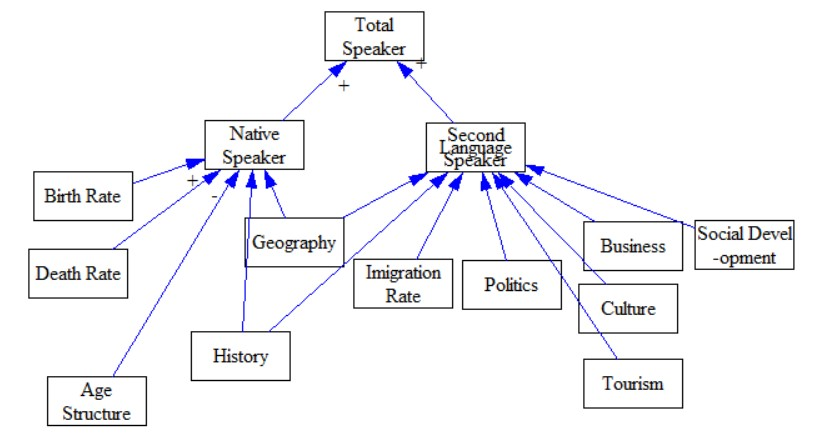
\includegraphics[width=15cm]{2.jpg}
\caption{Analysis of the Part I} \label{Analysis of the Part I}
\end{figure}
First, we model to predict the change of the number of  total speakers. The total speakers are mainly consist of two groups--- native speakers (L1) and second  (or third, etc.) language speakers (L2). The offspring of L1 are usually also L1. However, people learn the second language out of interest or the pressure of the school, that means their offspring are L2 uncertainly. Given the similarity between the number of L1 and population of a country,  we establish the age-dependent population model. It can help us quantitatively analyze the change of L1 precisely. The historic number of L1 can be found in our reference, and we choose one representative country to simulate the age structure of L1 and reproductive considerations for every language.\\
\indent For L2, the factor's influence is complicated. To establish a quantitative model precisely is hard. We determine to use statistic method to explore the relationship between the number of L2 and some factors.\\
\indent Second, we will predict the distribution of various languages in the future, we can draw the initial distribution in a world map. We can analogize a language to a country--- the distribution area of a language is its domain. If a country's comprehensive national strength is too weak, its powerful neighbor country invests its domain probably. As same, if a language's user decreases by a wide margin, its numerous-people-speak adjacent languages can `invest' its distribution range. Based on the above analogy, we establish the language distribution evolution model.\\
\indent Third, we study the emigration with regression analysis of time series in order to predict the situation of 50 years. and we use the same population to predict the number of the major area. Based on these data, we can draw the distribution and flow map of population over 50 years. Compare with this map and language distribution map, we can draw our conclusion. 

\subsection{Analysis of Part II}
First, we choose six international office based the following principals: 
\begin{enumerate}[1]
\item Internationalization: In these offices' service range, as many as kinds languages should be contained;
\item Advancement: the area located in these offices should be advanced. We estimate the degree of a country's advancement by Score which is related to GDP per capital, R \& D, etc. The weight vector is conferenced from the former research paper. 
\end{enumerate}
In the short term, we use the nowadays' data. In the long run we use the predicted future data.\\
\indent Second, for the sake of saving cost, we decrease the number of offices as a prerequisite to ensure the internationalization (at least cover ten languages). Because of the time complexity of the problem is too large, we use the genetic algorithm to find the solution. 

\section{Assumptions and Notations}
\subsection{Assumptions}
\begin{enumerate}[1]
\item We only consider the top-seventeen-languages. Due to more than half of the world population speaks the top ten languages. When it comes to the replacement, take seven more languages into consideration is reasonable. And the data of the top-seventeen-languages is complete basically. 
\item We neglect the influence of the factors whose effect is slight. 
\item We assume that the range of an office's service is a circle centered with its location. In the event, geographic and political conditions make it not a real circle. 
\end{enumerate}

\subsection{Notations}
\begin{table}[htbp]
\centering
\caption{The Definition of Variables}
\begin{tabular}{|c|l|}
\hline
Variable&Definition\\
\hline
L1&The number of native language speakers\\
\hline
L2&The number of second (or third, etc.) language speakers\\
\hline
\(p\)&Population density\\
\hline
\(r\)&Age\\
\hline
\(t\)&Time\\
\hline
\(f\)&Birth rate\\
\hline
\(\mu\)&Death rate\\
\hline
\(R\)&The radius of the range of service\\
\hline
\((\varphi_i, \theta_i)\)&The longitude and latitude of the city \(i\)\\
\hline
Score\(_i\)&The score of the city \(i\)\\
\hline
Kind&The kind of languages in the range of service region\\
\hline
\end{tabular}
\end{table}

\section{Language Distribution Evolution Model}
\subsection{Construction and Development of the Model}
The geographical and historical factor together determine the initial language distribution. For example, the Chinese terrain is flat in the north but rugged in the south. As a result, the dialects are fewer in the north than in the south. The Latin America has ever fallen into a colony of Portugal and Spain, so the people there speak Portuguese and Spanish. The birth and death rate, age structure, political, commercial, culture, tourist factor and the development of society affect the language distribution now. 

\subsubsection{Age-dependent Population Model}
Due to the great differences between birth rates and death rates of different age structures and long period of time, we introduce the population distribution function and density function. Based on the age-dependent population system, we can introduce a differential equation: 
  \[\frac{\partial p}{\partial r}+\frac{\partial p}{\partial t}=-\mu p\]
where \(p(r, t)\) is the population density function of age \(r\) and time \(t\). \(\mu(r, t)\) is the death rate of people aged \(r\) after \(t\) years. Combined with two define conditions, we can get the solution of the equation. 
\[p(r, 0)=p_0(r)\]
\[p(0, t)=f(0)\]
\begin{figure}[htbp]
\small
\centering
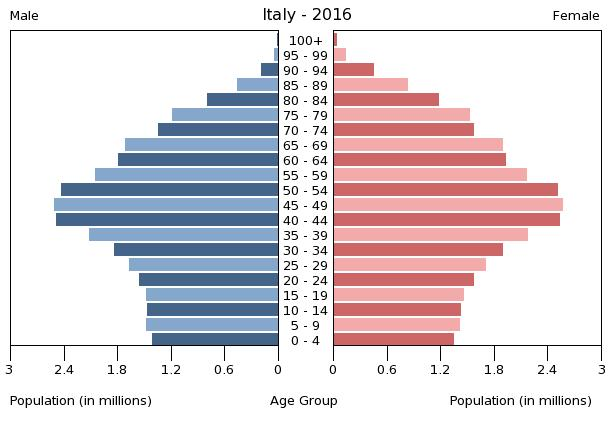
\includegraphics[width=8cm]{L11.jpg}
\caption{Fitting \(p_0(r)\) with Age Structure}
\end{figure}
Where \(p_0(r)\) means the initial population density function and \(f(t)\) is the birth rate. 
To simplify the solving process, we assume in the fifty years that the society will stay stable and the medical level is maintained, so the \(\mu(r, t)\) is equal to \(\mu(r)\). The solution is as follows: 
\[p(r, t)=\left\{
\begin{array}{lc}
p_0(t-r)e^{-\int\limits_{r-t}^{r}\mu(s)ds}&0\leqslant t\leqslant r\\
f(r-t)e^{-\int\limits_{0}^{r}\mu(s)ds}&t\geqslant r
\end{array}\right. \]
\[\textrm{L1}(50)=\int\limits_0^{\infty}p(r, 50)\textrm{d}r\]

\subsubsection{BP Neutral Network Prediction Model}
To simplify the model, we integrate and quantize the rest factors: 
\begin{enumerate}[1]
\item Normal population migration is represented as migration rate;
\item We use democracy index to indicate the degree of political civilization; 
\item As to commercial, cultural and tourist factors, we assume that the tertiary industry GDP can reflect them;
\item Social development can be shown in the total GDP. 
\end{enumerate}
We set the four indexes as input and L2 as output. By BP neutral network, we can speculate L2 and the four indexes over fifty years can be predicted by time series regression analysis. We can predict L2 over the future fifty years indirectly. 
\begin{figure}[htbp]
\small
\centering
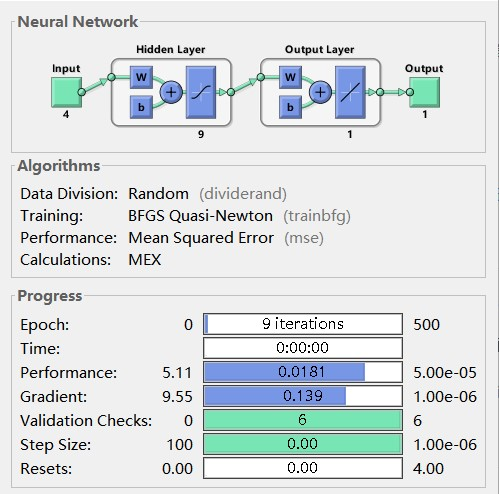
\includegraphics[width=8cm]{L21.jpg}
\caption{BP Neutral Network} \label{BP Neutral Network}
\end{figure}

\subsubsection{Probabilistic Model}
Given the communication and integration of different languages, we construct a model to reflect this dynamic process. We divide a map into pixels and introduce 2017 language distribution map as the initial map. We assume that language A will probably expand into the control region of language B when their influence areas are adjacent and the number of A speakers is more than that of B speakers. The possibility formulation is as follows:
\[P\{\textrm{A `invest' B}\}=\left\{
\begin{array}{lc}
1-\dfrac{L_B}{L_A}&L_A\geqslant L_B\\
0&L_A\leqslant L_B
\end{array}\right. \]
\[L=\textrm{L1}+\textrm{L2}\]
Where \(L_A\) and \(L_B\) are the number of A and B speakers. The assumption is rational because when \(L_A \rightarrow\infty\) or \(L_B=0\), that means A has replaced B in fact.\\
\indent Based on the above two models, we can predict the number of total speakers for each language every year in the future. After fifty iterations, we can get language distribution map over fifty years.\\
\indent And we also utilize the historic data predict the number of emigrants and local people in each area. We can plot population distribution and emigrant tendency map.

\subsection{Results of the Model}
\begin{figure}[htbp]
\small\centering
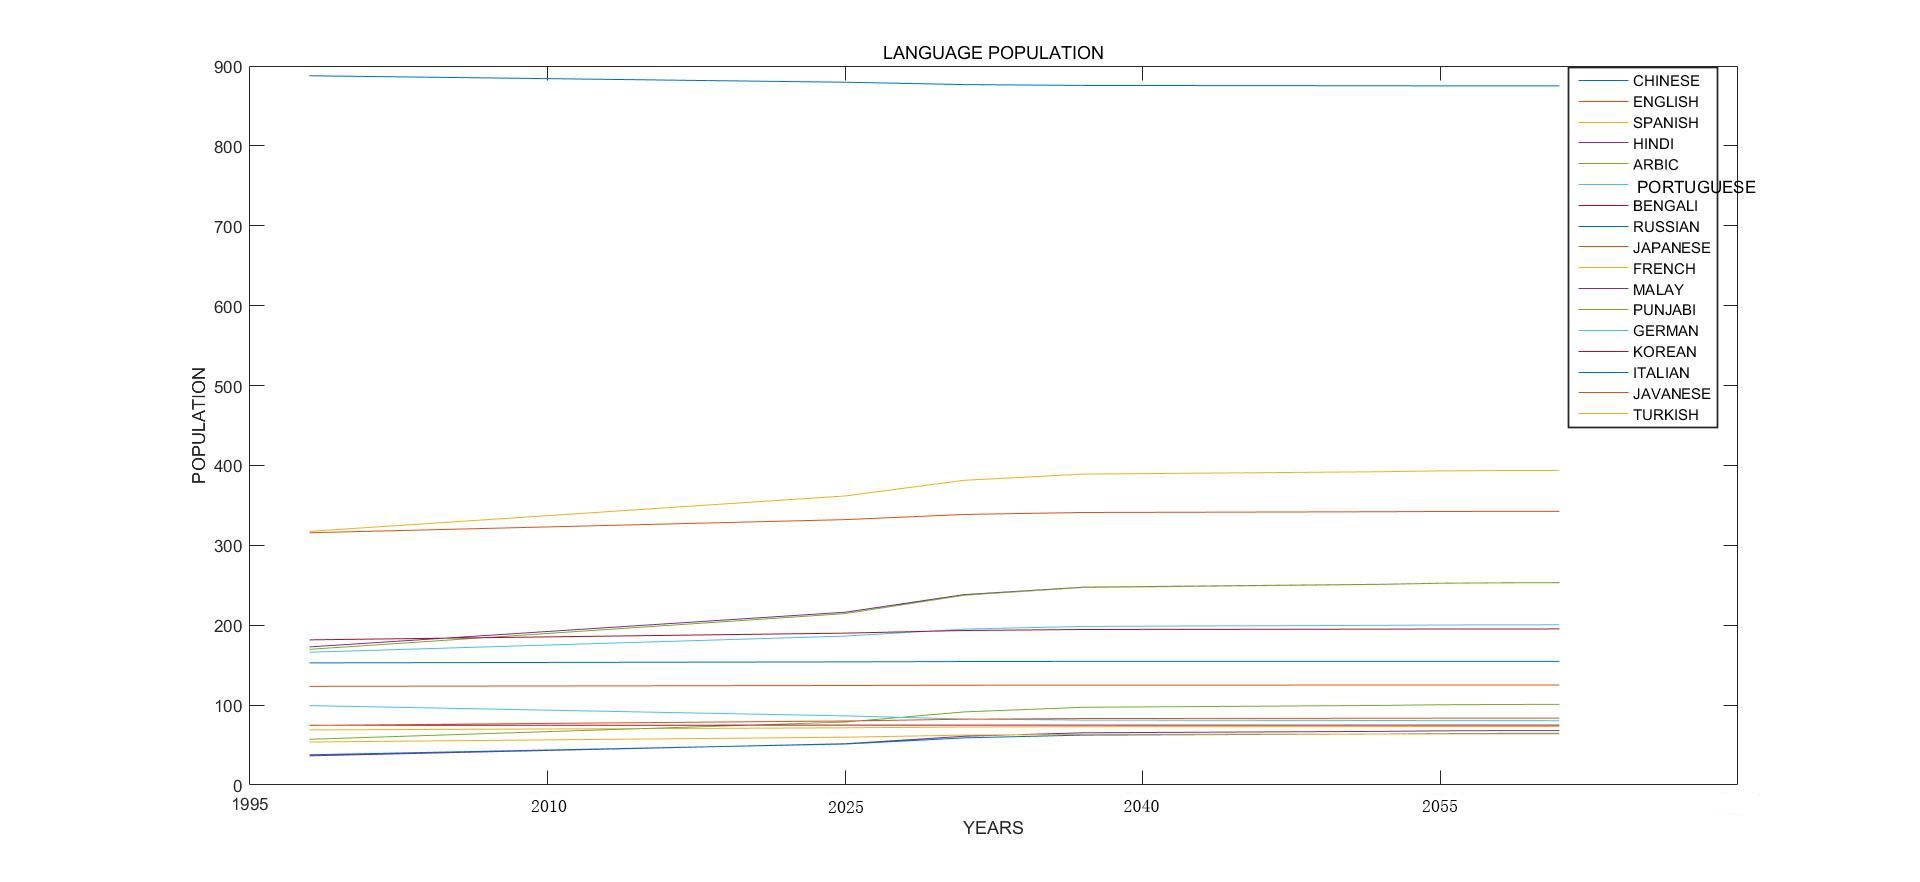
\includegraphics[width=10cm]{L12.jpg}
\caption{Prediction of L1 (Unit:  million)}
\end{figure}
We just display the prediction of language whose native speakers are more than fifty million. L1 of Chinese and Bengali decrease evidently. Because Chinese and Bengali degree of aging will reduce their native population in the future. Few languages' L1 ascend in a small amplitude, such as Punjabi and Spanish. By speculating, this phenomenon is related to high birth rate of Pakistani and Latin American. The change of other languages is not obvious.\\
\indent We use twenty groups of date from 2015 to 2017 to train neutral network and four groups of date in 2017 to check neutral network. 
\begin{figure}[htbp]
\centering
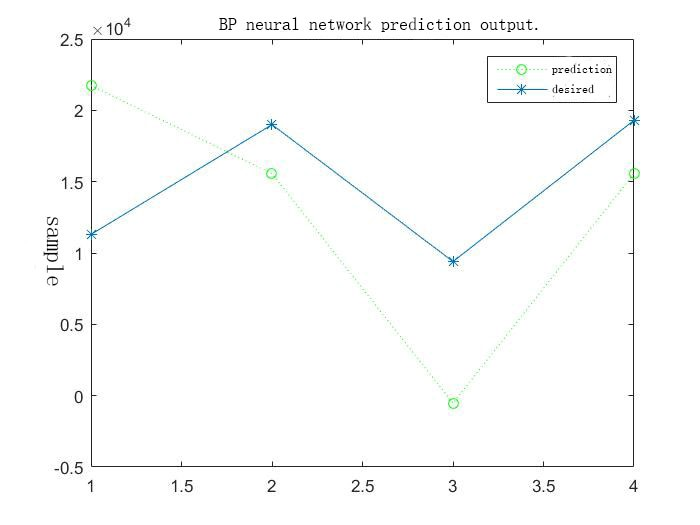
\includegraphics[width=8cm]{L22.jpg}
\caption{The Prediction Output of BP Neutral Network}
\end{figure}
\begin{figure}[htbp]
\centering
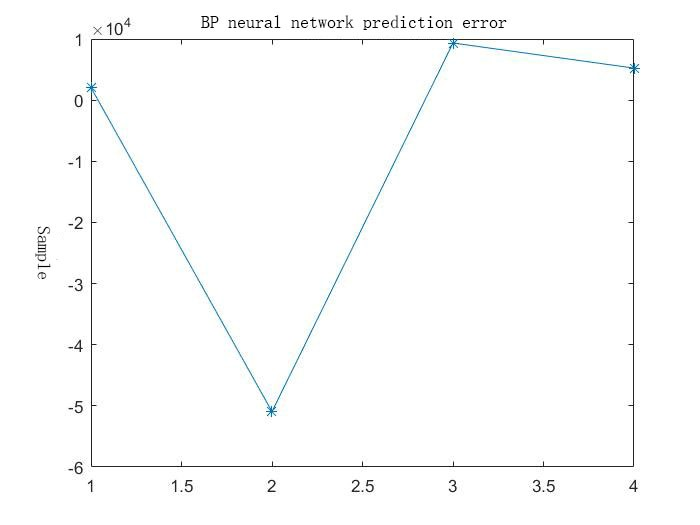
\includegraphics[width=8cm]{L23.jpg}
\caption{The Prediction Error of BP Neutral Network}
\end{figure}
The results of test suggest BP neutral network have splendid capability to predict L2.
\begin{table}[htbp]
\centering
\caption{Prediction of L2 (Unit:  million)}
\begin{tabular}{|c|c|c|c|c|c|}
\hline
Language&Democracy index&Tertiary GDP&Total GDP&Mobility Ratio&L2\\
\hline
Chinese&3. 14&8124531.09&15358281. 00&0. 63&224\\
\hline
English&8. 05&19085756.06&23946996. 00&4. 33&642\\
\hline
Spanish&8. 3&1126867.962&1552160. 00&-1. 95&90\\
\hline
Hindi&7. 74&1553932.934&2730990. 00&0. 12&134\\
\hline
Arabic&2. 75&189625.0415&476444. 00&-0. 32&135\\
\hline
Brazilian&7. 79&1457970.955&2169600. 00&-0.02&8\\
\hline
Bengali&5. 73&52150.71795&235000. 00&-4.2&15\\
\hline
Russian&3. 31&942218.0592&1567750. 00&1.83&115\\
\hline
Japanese&7. 96&3663033.983&5130300.00&0&1\\
\hline
French&8. 82&2225046.947&2788280.00&1.22&155\\
\hline
Malay&7. 03&380610.01&980953.00&-0. 28&210\\
\hline
Panjabi&5&60672.04436&310500.00&-1.11&50\\
\hline
\end{tabular}
\end{table}
\begin{table}[htbp]
\centering
\caption{Language Rank (Unit:  million)}
\begin{tabular}{|c|c|c|c|c|c|c|c|c|}
\hline
\multirow{3}{*}{\diagbox[dir=NW,width=8em]{Name}{Value}{Time}}&\multicolumn{4}{c|}{2017}&\multicolumn{4}{c|}{2067}\\
\cline{2-9}
&\multicolumn{2}{c|}{Native}&\multicolumn{2}{c|}{Total}&\multicolumn{2}{c|}{Native}&\multicolumn{2}{c|}{Total}\\
\cline{2-9}
&Number&Rank&Number&Rank&Number&Rank&Number&Rank\\
\hline
Mandarin Chinese&897&1&1090&1&865&1&1089&1\\
\hline
English&371&3&983&2&392&3&1034&2\\
\hline
Hindustani&329&4&544&3&350&4&484&4\\
\hline
Spanish&436&2&527&4&466&2&556&3\\
\hline
Arabic&290&5&422&5&312&5&447&5\\
\hline
Malay&77&15&281&6&80&11&290&6\\
\hline
Russian&153&8&267&7&138&9&253&8\\
\hline
Bengali&242&6&261&8&254&6&269&7\\
\hline
Portuguese&218&7&229&9&227&7&235&9\\
\hline
French&76&17&229&9&79&12&232&11\\
\hline
Punjabi&148&9&148&11&182&8&234&10\\
\hline
Japanese&128&10&129&12&135&10&136&12\\
\hline
\end{tabular}
\end{table}
\begin{figure}[htbp]
\centering
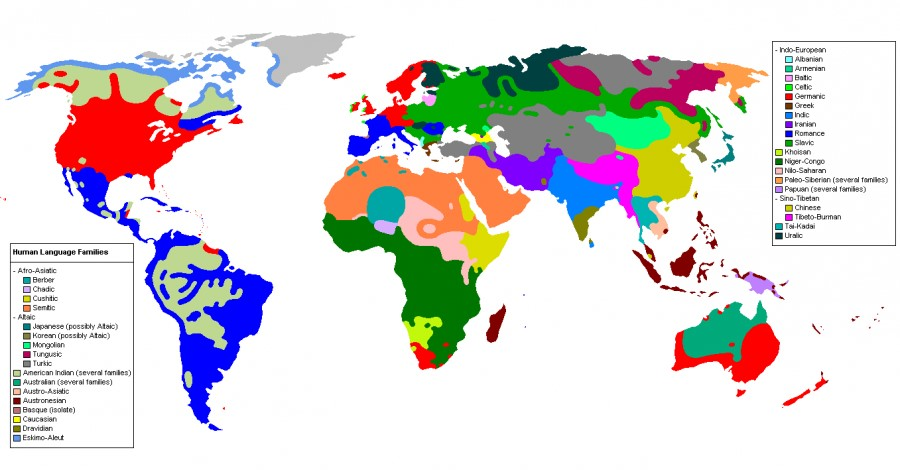
\includegraphics[width=10cm]{L31.jpg}
\caption{Initial Language Distribution Map}
\end{figure}\\
\indent We use the number of total speakers to model the language distribution evolution trend prediction model. For other few-people-speak languages, we estimate their total speakers' numbers above fifty million.\\
\begin{figure}[htbp]
\centering
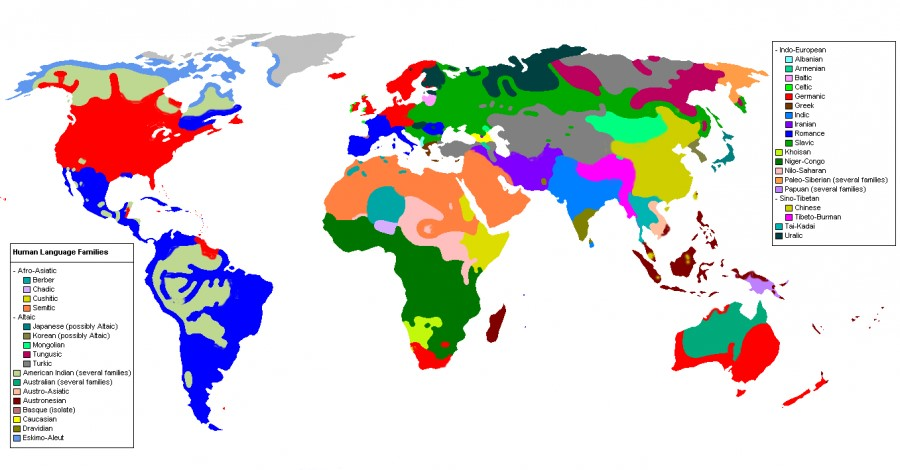
\includegraphics[width=10cm]{L32.jpg}
\caption{Future Language Distribution Map}
\end{figure}
\begin{figure}[htbp]
\centering
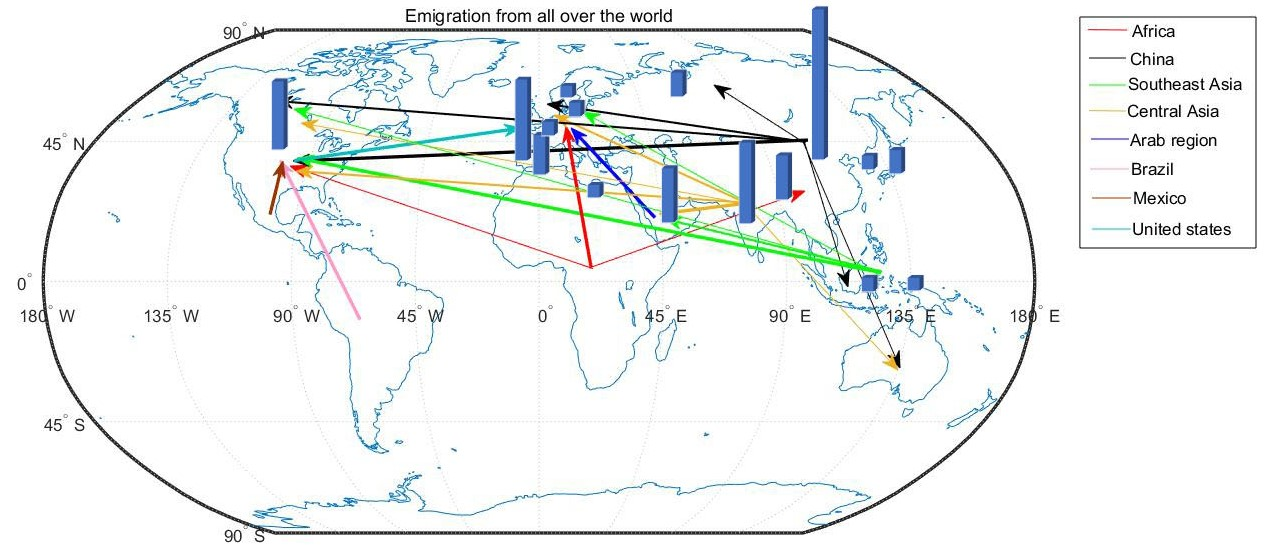
\includegraphics[width=10cm]{E.jpg}
\caption{Population Distribution and Emigrant Tendency Map}
\end{figure}
\indent By comparison, language distribution is related to the population and emigration. 

\subsection{Data Analysis}
\begin{enumerate}[A]
\item The figure 8 has shown us the distribution of various languages over fifty years. It is estimated that linguistic diversity is under destruction. The L1 of English vary obscurely but L2 rise up in the future. It explains why the range of English distribution expand evidently. Although the L1 of Chinese descend in the future since Chinese population shrinks over time, L2 ascend. In general, the range of Chinese distribution will increase. The L1 of Spanish rise, but L2 is in decline. In spite of this, the total speakers remain to go up. The region of Spanish spreads in some degree. The number of Bengali native speakers will decline and the change of L2 maintain steady. It is estimated that Bengali's region will shrink. Other languages' change is unapparent.
\item The figure 4 has shown us the number of some native languages speakers over fifty years. The table 3 have shown us the number of some total speakers over fifty years. Punjabi can replace French as the tenth on the number of total language speakers. By deducing, this phenomenon has relation with its high birth rate. On the contrary, the most of developed countries including France are suffering from negative population growth. 
\item The figure 9 has shown us population and emigrant tendency. The geographic distributions of these languages change over this same period of time. Language expansion is centered with the area where population is concentrated, in the opposite direction of emigration approximately. A bit exception maybe results from politic reason---such as emigration policies.
\end{enumerate}

\subsection{Robustness Analysis}
We change the four inputs in BP neutral network into three to check whether there exists absolute dependence to one input. Results suggest that the prediction error will increase and absolute dependence does not exist. 
\begin{figure}[htbp]
\centering
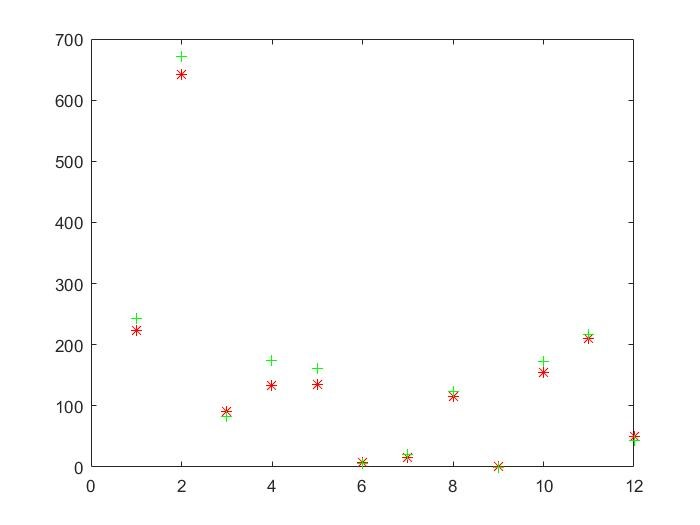
\includegraphics[width=10cm]{V.jpg}
\caption{Robustness Analysis}
\end{figure}

\section{Location Optimization Model}
\subsection{Construction and Development of the Model}
\subsubsection{0-1 Multi-objective Programming Model}
We choose the kind of languages in the range of a city's service region as the city's degree of internationalization. The range of a city's service region is a circle centered with \((\varphi_j, \theta_j)\) and its radius is \(R\). The \((\varphi_j, \theta_j)\)is the location of the city which is a consistent one-to-one match with a pixel of the map. The \(R\) is usually about 2000 kilometers for a multinational service company. It corresponds to fifty pixels in the map.\\
\indent We choose the score as the city's degree of advance. The score has a positive correlation to FDI. The formulation of score and the provident of its positive correlation to FDI come from the reference [2].
\begin{table}[htbp]
\centering
\caption{The Indexes About Score}
\begin{tabular}{|c|c|l||}
\hline
Variable&Full Name&Mean\\
\hline
avgGDP&GDP per capital&Reflect market capacity and total demand.\\
\hline
wage&Wages&Reflect labor cost.\\
\hline
patent&Patent&Reflect the innovation ability.\\
\hline
hr&Human resources&Reflect the human capital.\\
\hline
rd&Research and development&Reflect the technical level.\\
\hline
FDI&Foreign direct investment&Reflect the financial resources.\\
\hline
\end{tabular}
\end{table}
\[\textrm{max }P_1\textrm{Kind}+P_2\sum\limits_{i=1}^{n}X_i\textrm{Score}_i\]
\[\textrm{s. t. }\left\{
\begin{array}{l}
\textrm{Kind}: \textrm{the kind of languages in the range of service region of city }j\textrm{ for }X_j=1\\
\textrm{Score}_i=\beta_0+\beta_1ln\textrm{avggap}_i+\beta_2ln\textrm{wage}_i+\beta_3ln\textrm{patent}_i+\beta_4ln\textrm{hr}_i+\beta_5\textrm{fdiagg}_i+\beta_6ln\textrm{rd}_i\\
P_1\gg P_2\\
X_i\in\{0, 1\}\\
\textrm{card}\{i: X_i=1\}=6
\end{array}\right. \]
\indent The \(X_i\) is a 0-1 variable. If and only if we set the office in the city \(i\), \(X_i=1\). \(P_1\gg P_2\)means that the importance of internationalization is much greater than the advancement, because the company's original intention is becoming international. The variable \(n\) is the numbers of cities which can be chosen. Given the company already have offices in New York and Shanghai, we give up selecting other cities in America and China. Because the problem is a combinatorial optimization problem---the time complexity \(T(n)\) increase rapidly with \(n\), we just choose twenty-five cities. 
\begin{figure}[htbp]
\centering
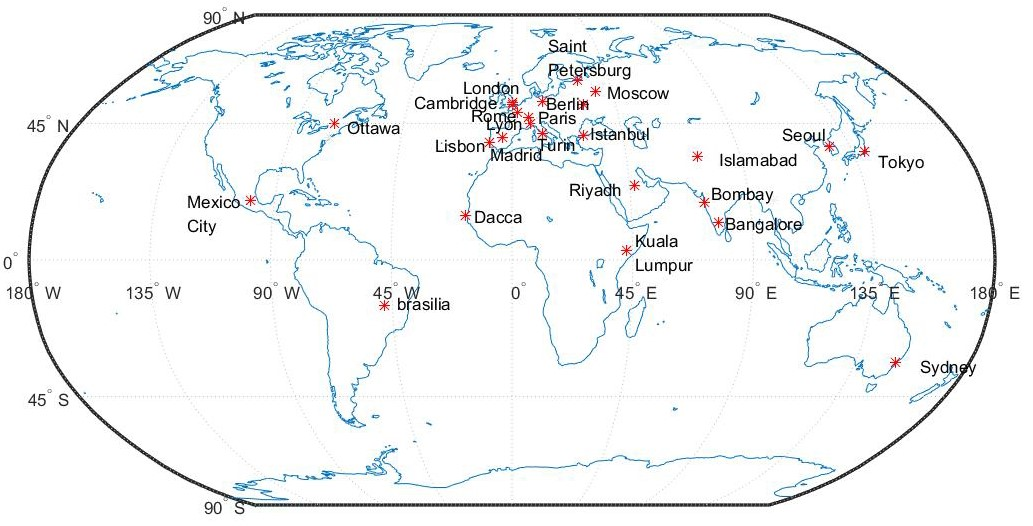
\includegraphics[width=10cm]{A1.jpg}
\caption{The Cities Which We Select}
\end{figure}\\
Even so, to solve this problem needs too much time. We have to select heuristic algorithm.\\
\[T(n)=\Theta(\left(
\begin{matrix}
n\\
6
\end{matrix}\right))=\Theta(n^r), r\approx5. 97\]
\[\left(
\begin{matrix}
25\\
6
\end{matrix}\right)=177100\]
And the problem is multi-objective programming problem. We use sequential algorithm to decompose the problem into the two programming problems.
\[\textrm{max }\textrm{Kind}\]
\[\textrm{s. t. }\left\{
\begin{array}{l}
\textrm{Kind}: \textrm{the kind of languages in the range of service region of city }j\textrm{ for }X_j=1\\
X_i\in\{0, 1\}\\
\textrm{card}\{i: X_i=1\}=6
\end{array}\right. \]
\[\textrm{max Score}=\sum\limits_{i=1}^{n}X_i\textrm{Score}_i\]
\[\textrm{s. t. }\left\{
\begin{array}{l}
\textrm{Score}_i=\beta_0+\beta_1ln\textrm{avggap}_i+\beta_2ln\textrm{wage}_i+\beta_3ln\textrm{patent}_i+\beta_4ln\textrm{hr}_i+\beta_5\textrm{fdiagg}_i+\beta_6ln\textrm{rd}_i\\
X_i\in\{0, 1\}\\
\textrm{card}\{i: X_i=1\}=6\\
\{i: X_i=1\}\textrm{ make Kind maximal in the above problem}
\end{array}\right. \]
We choose genetic algorithm without variation. 
\begin{figure}[htbp]
\centering
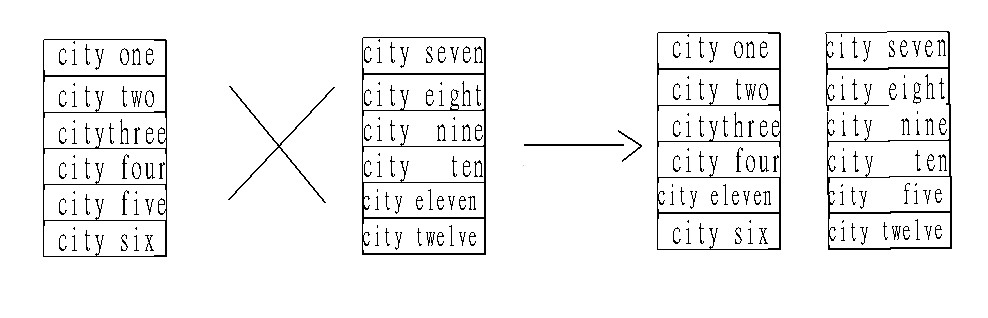
\includegraphics[width=8cm]{G.jpg}
\caption{Parent Sample Generate Child Sample}
\end{figure}
\begin{enumerate}[1]
\item Generate 400 sample randomly. Every sample consists of six cities. 
\item Calculate their Kind. 
\item Rank these samples by their Kind. 
\item Retain the first one hundred. 
\item Pair them off. 
\item Exchange their components to generate 400 new samples. 
\item Return the second step until the similarity is adequate (the number of the same sample is more than 200) or the number of iterations is more than 100. 
\item Search the sample whose number is the largest. Output it. 
\end{enumerate}
We repeat running the program fifty times and calculate the fifty results' Score. We recommend the scheme whose Score is the largest. We use the data in 2017 to calculate short-term results and the data we predicted over the future fifty years to estimate long-term results.

\subsubsection{0-1 Programming Model}
Out of the similarity to the above model, we choose the same indexes. The only difference is that we just need the range of service region cover ten languages---it represents  that the company is international adequately. As a presupposition to be international adequately, we choose different variable \(k\)---the number of offices to calculate the total score. 
\[\textrm{max Score}=\sum\limits_{i=1}^{n}X_i\textrm{Score}_i\]
\[\textrm{s. t. }\left\{
\begin{array}{l}
\textrm{Kind}: \textrm{the kind of languages in the range of service region of city }j\textrm{ for }X_j=1\\
\textrm{Score}_i=\beta_0+\beta_1ln\textrm{avggap}_i+\beta_2ln\textrm{wage}_i+\beta_3ln\textrm{patent}_i+\beta_4ln\textrm{hr}_i+\beta_5\textrm{fdiagg}_i+\beta_6ln\textrm{rd}_i\\
\textrm{Kind}\geqslant 10\\
X_i\in\{0, 1\}\\
\textrm{card}\{i: X_i=1\}=k\leqslant6
\end{array}\right. \]
The total cost will decrease with the decrease of \(k\). However, the total score is also in decline. So, we will recommend to choose the scheme which has the maximal average score. 
\[\textrm{avgScore}(k)=\frac{\textrm{Score}(k)}{k}\]

\subsection{Results of the Model}
\begin{figure}[htbp]
\centering
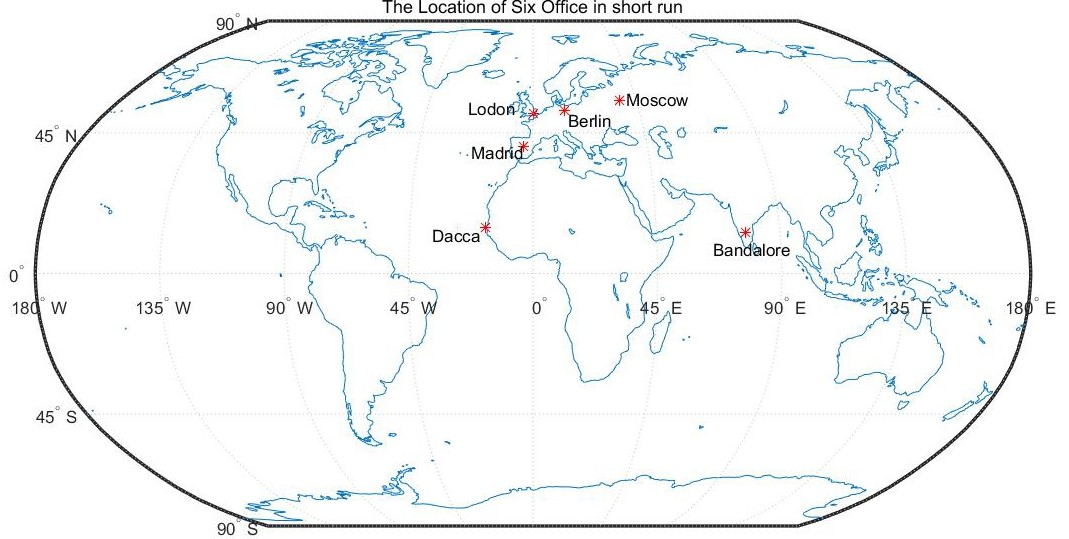
\includegraphics[width=10cm]{B1.jpg}
\caption{The Location of Six Offices in the Short Term}
\end{figure}
\begin{figure}[htbp]
\centering
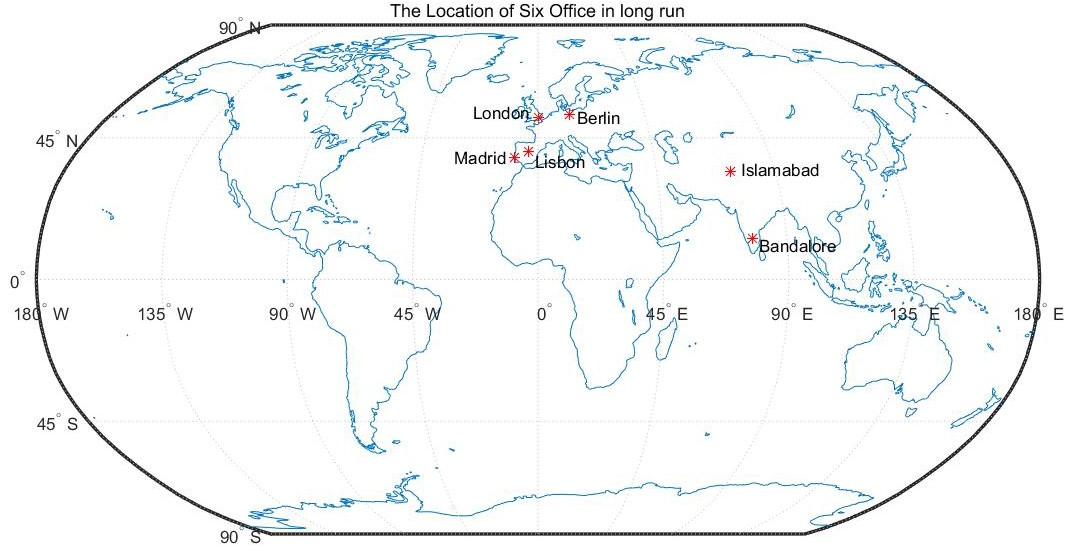
\includegraphics[width=10cm]{B2.jpg}
\caption{The Location of Six Offices in the Long Run}
\end{figure}
The result in a short term and a long run is slightly different. 
\begin{table}[htbp]
\centering
\caption{The Result to Different Variable \(k\) in the long run}\label{The Result to Different Variable k}
\begin{tabular}{|c|c|c|c|c|c|c|c|}
\hline
\(k\)&6&5&4&3&2&1&0\\
\hline
Score&145. 362&122. 635&96. 8&0&0&0&0\\
\hline
avgScore&24. 227&24. 527&24. 200&0&0&0&0\\
\hline
\end{tabular} 
\end{table}\\
\indent
0 means no answer. When k=5, avgScore is maximal. So we recommend the below scheme. 
 \begin{figure}[htbp]
\centering
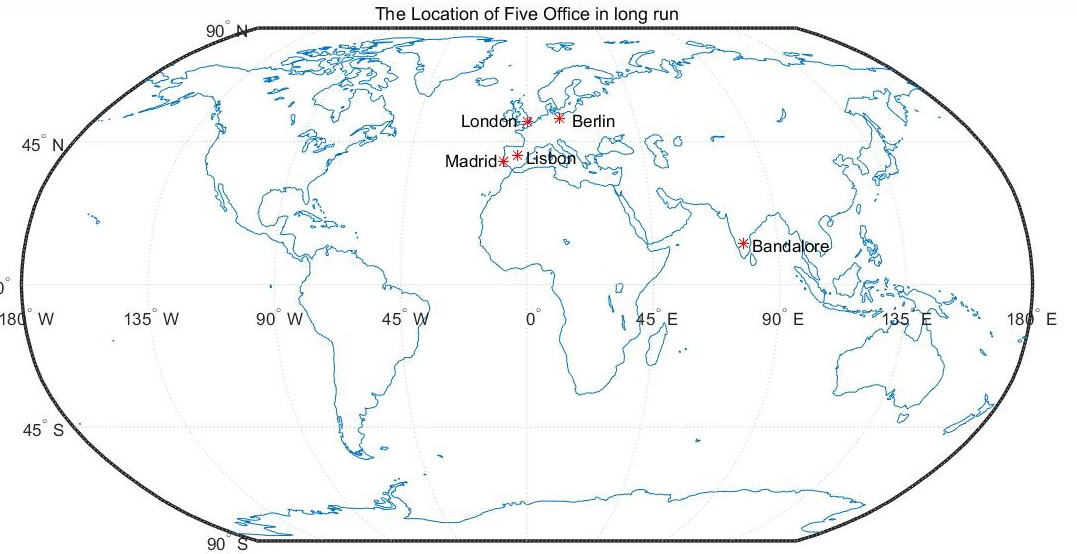
\includegraphics[width=10cm]{B3.jpg}
\caption{The Location of Five Offices in the Long Run}
\end{figure}

\subsection{Data Analysis}
\begin{enumerate}[A]
\item It is obvious that the recommendations will be different in the short term and in the long run. As shown in figure 12 and 13, we select London (England), Dacca (Bengal), Berlin (German), Moscow (Russia), Madrid (Spain), Bangalore (Indian) in the short term while choosing London (England), Berlin (German), Madrid (Spain), Bangalore (Indian), Islamabad (Pakistan), Lisbon (Portugal) in the long run. We deduce that the Islamabad being selected in the future long run is related to the increasing number of the Punjabi speakers. Furthermore, due to the decrease of Bengali speakers, the Dacca fails to be chosen. 
\item In order to save the company resources, we try the variable \(k\) from five to zero. After running the program, we find that when \(k\) is equal to three, two, one, the internationalization goal cannot be achieved. We calculate the average score when k is equal to six, five and four and find that the average score gets the biggest result when \(k=5\). Thus, we suggest the company to choose five new offices. 
\end{enumerate}

\subsection{Validation and Sensitivity Analysis}
\subsubsection{Sensitivity Analysis}
We can change the radium \(R\) to observe whether the solution will change. We change \(R\) from 50 pixels at the step of 10 pixels. The results suggest when the variable \(R\geqslant80\) we can find many different schemes. But we cannot determine whether we have find the best solution because of the heuristic algorithm.

\subsubsection{Validation of the Model}
\indent We choose the two companies---Microsoft Corporation and McKinsey \& Company. Their fields are technology and consulting respectively. In fact, the number of their branch office far exceed six. So, we just choose the most important research institutes or the earliest several offices to certificate our scheme.\\ \begin{figure}[htbp]
\small\centering
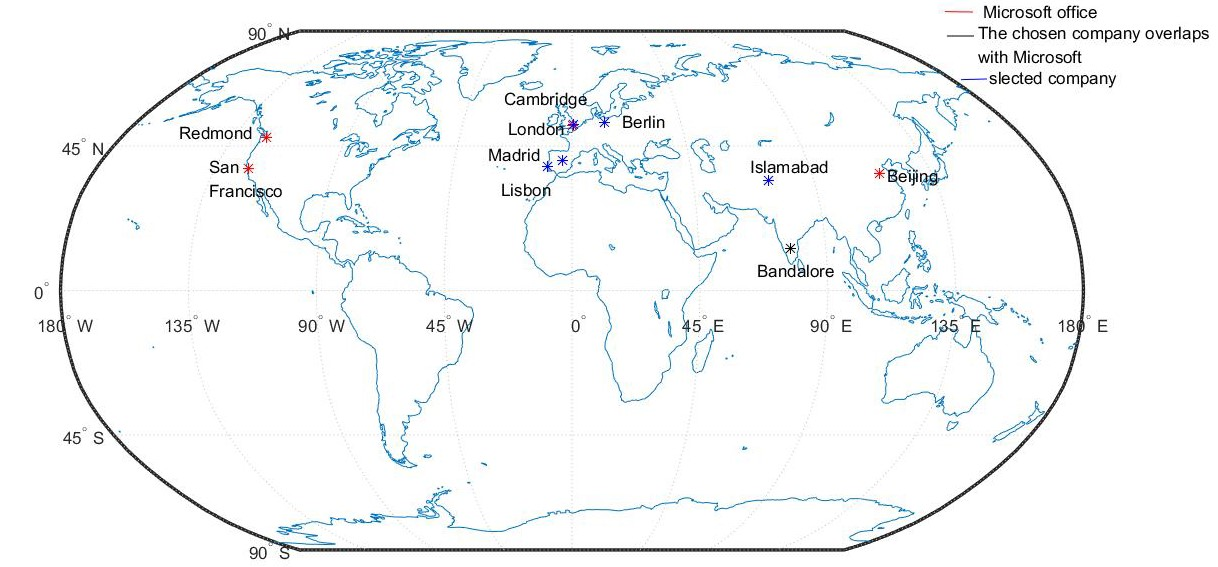
\includegraphics[width=10cm]{M1.jpg}
\caption{The Six Research Institutes of Microsoft Corporation}
\end{figure}
\begin{figure}[htbp]
\small\centering
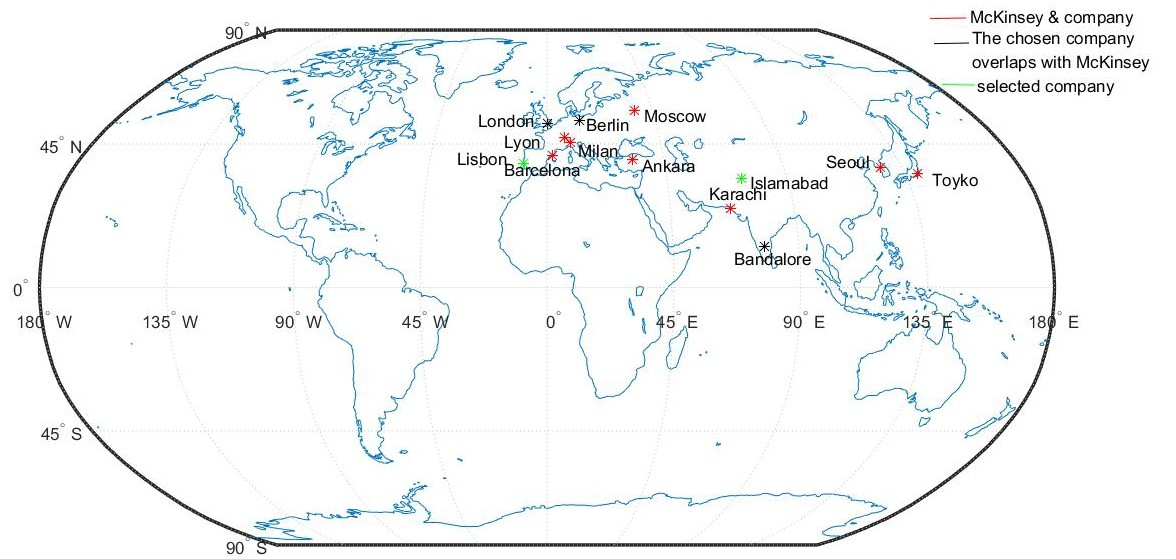
\includegraphics[width=10cm]{M2.jpg}
\caption{The Earliest Branch Office of McKinsey \& Company}
\end{figure}\\
\indent We can see the coincidence between the most of cities which we choose and their branch offices. It proves that our model has some degree of reliability in reality. 

\section{Strengths and Weaknesses}
\subsection{Strengths}
\begin{enumerate}[1]
\item We derive our model from various affecting factors and limit our use of assumptions. In every case where an assumption is required, we substantiate it with evidence and reasoning that illustrates why the assumption is valid. Thus, our model is credible and robust. 
\item We take full accounts of various factors that affect the profits of the company. Under the premise of accomplishing the goal of internationalization, we construct a score function that reflects the company's profit demands. Such a score function gives our selection great flexibility:  if more factors are taken into considerations, we can simply add the contribution of that factor to the function. This flexibility is of great value in practice since the requirements of the company may vary at different times. 
\item The trends of language distribution returned  by  our first model  tie  in  with  those given by previous studies  by experts in the  field. 
\end{enumerate}

\subsection{Weaknesses}
\begin{enumerate}[1]
\item Language's extension is a completed process with many affecting factors. Despite we take some notable factors into consideration, accuracy still could be increased through a detailed entering of the course with more parameters. 
\item The age-dependent population model is too simple. We ignore the changes of the death rate and assume it is a constant. Thus, it is hard to precisely predict the trends of native language speakers. 
\item Due to the restriction of the hardware, we do not have enough time to solve location optimization model. Heuristic algorithm cannot ensure our answer is the best solution. Our genetic algorithm without variation is easy to fall into the local optimal solution not the global optimal solution. 
\end{enumerate}

\section{Future Work}
\subsection{Future Development of the Model}
\begin{enumerate}[1]
\item If gotten the further support of enough data like the changes of death rate, our prediction about the future number of various languages will be more precise and results in more accurate conclusion about trends of language distribution. 
\item As to our language distribution evolution model, the probability whether language A will expand into the area of language B is determined through data fitting. However, the probability can be calculated by various factors such as economy, culture and so on. Thus the model can be more valid and robust. 
\item Usually a company's development demands will vary from time to time, so it is more reasonable to establish flexible standards set up to accommodate different situations to optimize the location selection. 
\end{enumerate}

\subsection{Extension of the Model}
When it comes to the formulation of national policies and the input of national resources, the comprehensive urban development index of different cities can be a vital reference factor. Our score system can be extended through selecting different parameters to apply to the demand. 

\section{A Memo to the Chief Operating Officer}
To: The Chief Operating Officer\\
From: Models\\
Re: Open Office Mathematically\\\\
Dear Sir/Madam:\\\\
\indent We have heard of your company's future planning of internationalization. We offer you our assistance. We are a team of students who have dedicated four intense days to predict the future number and geographical distribution of various languages. While many have been working on this problem for years, we feel our approach will give your company the extra edge you are seeking.\\
\indent For the crucial goal of achieving internalization, we first make predictions of future language distribution. Total speakers' numbers is divided into two groups--- native speakers and second-language speakers. The number of native speakers is calculated through age-dependent population system and that of second-language speakers is incorporated with extensive demographic data by BP neutral network. Based on the total speakers' number, we construct a language distribution evolution trend prediction model. In our prediction, the area of English will increase greatly and that of Bangladesh will shrink. As to Japanese and Russian, the region will maintain initial state. The detailed distribution is shown in our paper.\\
\indent On the basis of the prediction of various language speakers' number and distribution, we formulate the location optimization model to help make the selections. Allowing for the fact that the company's profit demands, we set up a score system related to the cities' financial, innovative factors and so on. 
The goal of internalization is quantized into the total number of languages. The service region of a city is supposed as \(r\). If the region of a language is within \(r\), we count this language into the total number. On the premise of internalization, we select the locations whose scores are higher. In the short term, we select London (England), Dacca (Bengal), Berlin (German), Moscow (Russia), Madrid (Spain), Bangalore (Indian) while selecting London (England), Berlin (German), Madrid (Spain), Bangalore (Indian), Lisbon (Portugal) and Islamabad (Pakistan) in the long run.\\
\indent For the sake of saving resources, we try to choose less offices to get higher average scores while maintain internalization. Through calculation, we find that the average scores are the highest when we choose five offices, located at London (England), Bangalore (Indian), Madrid (Spain), Berlin (German) and Lyon (France).\\
\indent In view of possible various demands of your company during different times, our model focuses on the flexibility and can apply for different demands through introducing other factors into our scores system.\\
\indent We have given you only a taste of what our model can do. We hope you will agree that contracting for our services will be of the highest benefit to your esteemed company.\\\\
Sincerely\\
Models

\newpage
\begin{thebibliography}{99}
\bibitem{1}M. A. F Gomes. Geometrical aspects in the distribution of languages and urban settlements[J]. Physica A:  Statistical Mechanics and its Applications, 2001, 295(1). Publishing Company, 1984-1986.
\bibitem{2}Yongli Wang. The study of influence factors on the location choice of multinational enterprises[D]. Nankai University, 2010.
\bibitem{3}\url{http://fairlanguages.com/what-are-the-top-5-world-languages-in-2050}
\bibitem{4}\url{https://www.ethnologue.com/archive}
\bibitem{5}\url{https://en.wikipedia.org/wiki/List_of_languages_by_number_of_native_speakers}
\bibitem{6}\url{https://data. worldbank. org. cn/}
\bibitem{7}\url{https://en. wikipedia. org/wiki/Microsoft_Research}
\bibitem{8}\url{https://www.mckinsey. com/locations}
\end{thebibliography}

\begin{appendices}
\section{Code}
Here are simulation programs we used in our model as follow.\\
\indent
\lstinputlisting[language=Matlab]{./code/PredictionOfL1.m}
\lstinputlisting[language=Matlab]{./code/PredictionOfL2.m}
\lstinputlisting[language=Matlab]{./code/LanguageDistributionEvolutionModel.m}
\lstinputlisting[language=Matlab]{./code/RobustnessAnalysis.m}
\lstinputlisting[language=Matlab]{./code/Cities.m}
\lstinputlisting[language=Matlab]{./code/GeneticAlgorithm.m}

\section{Data}
Here is part of date we used in our model as follow.\\
\indent
\begin{figure}[htbp]
\small\centering
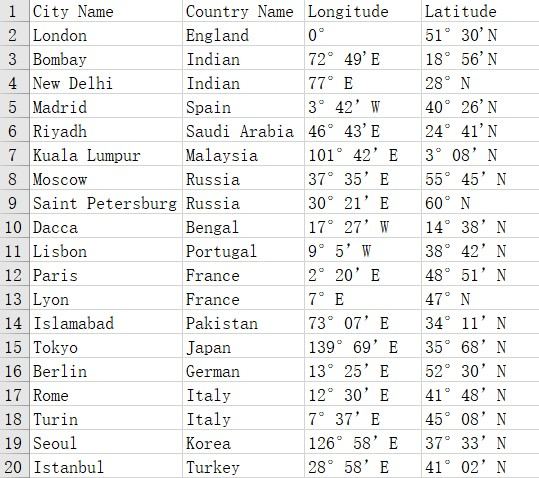
\includegraphics[width=8cm]{d0.jpg}
\caption{Cities}
\end{figure}
\begin{figure}[htbp]
\small\centering
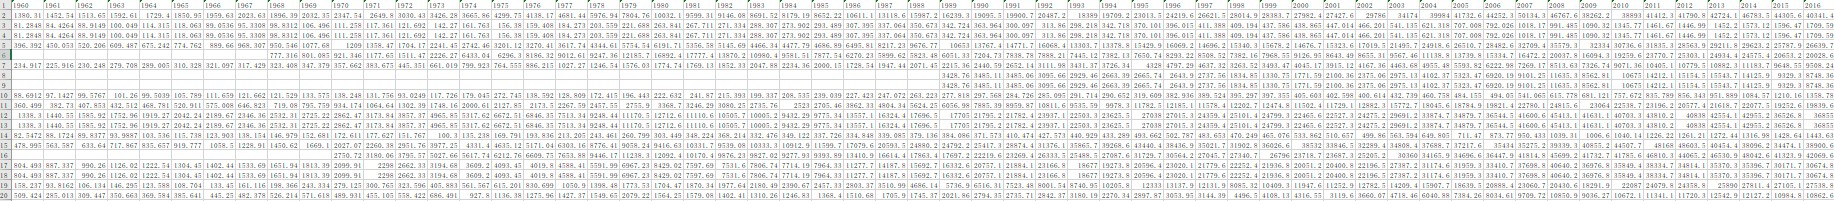
\includegraphics[width=15cm]{d1.jpg}
\caption{avgGDP}
\end{figure}
\begin{figure}[htbp]
\small\centering
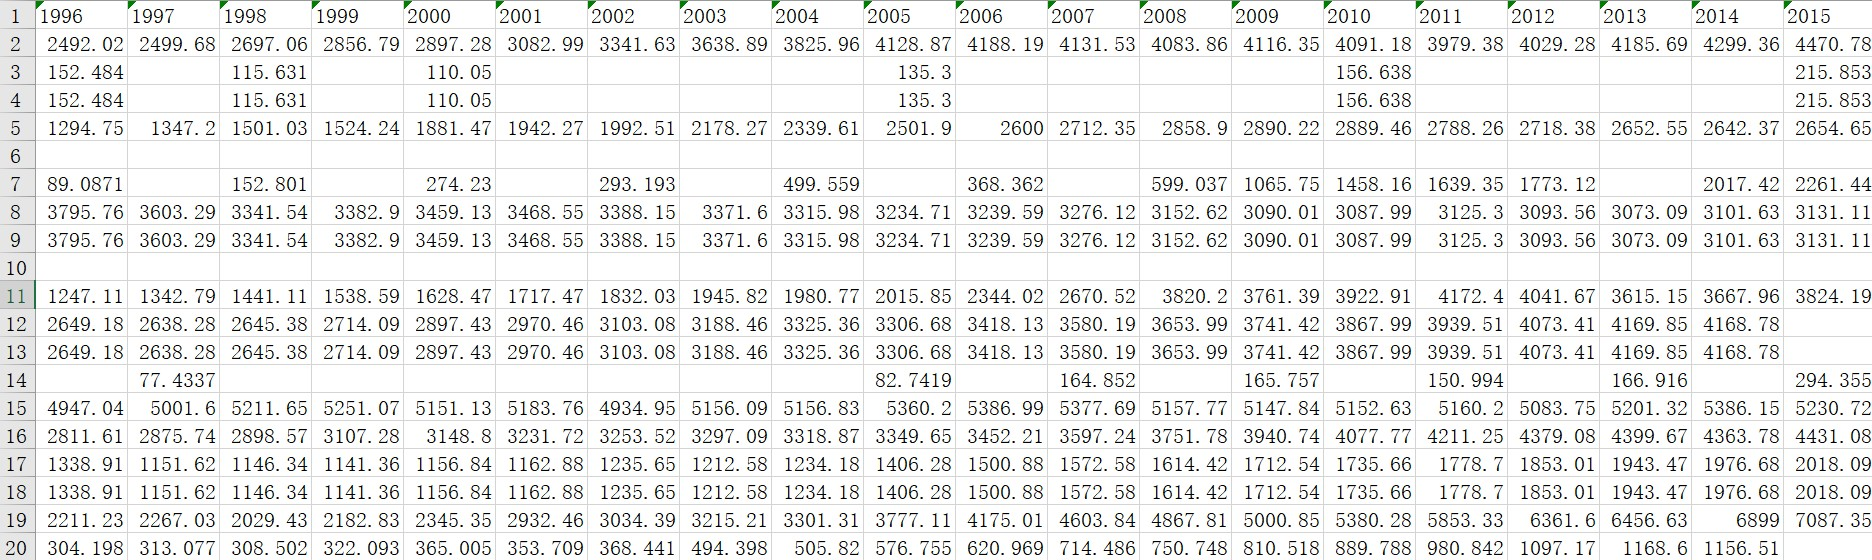
\includegraphics[width=10cm]{d2.jpg}
\caption{R\&D}
\end{figure}
\begin{figure}[htbp]
\small\centering
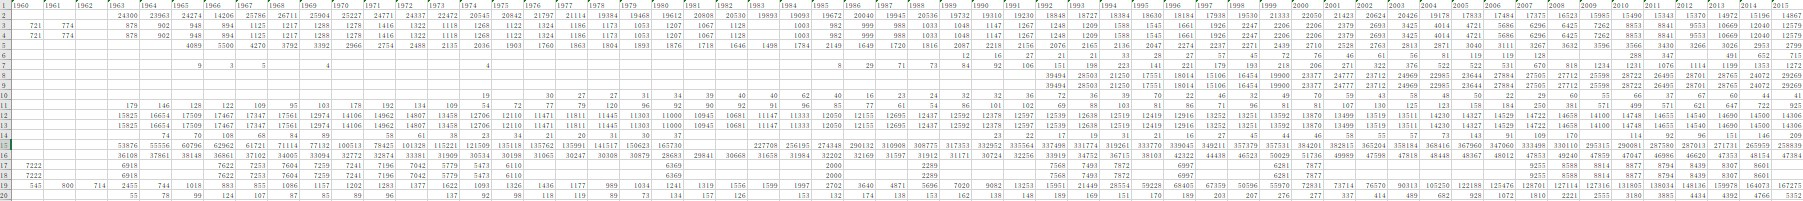
\includegraphics[width=15cm]{d3.jpg}
\caption{FDI}
\end{figure}
\end{appendices}
\end{document}
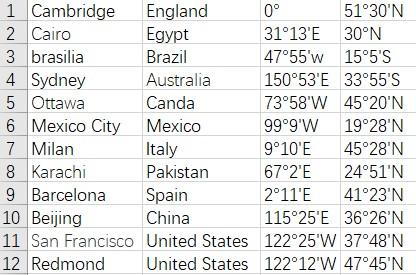
\includegraphics[width=15cm]{d4.jpg}
\caption{Score}
\end{figure}
\end{appendices}
\end{document}
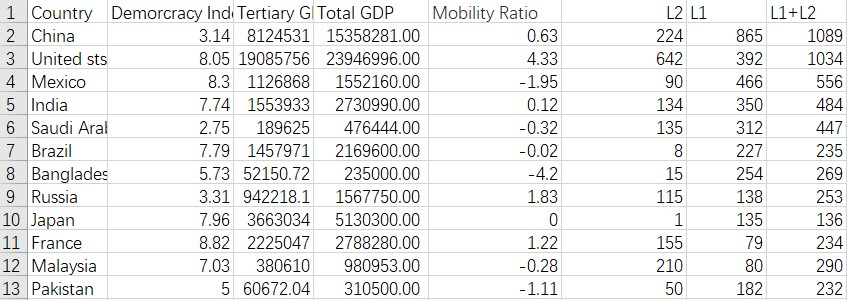
\includegraphics[width=15cm]{d5.jpg}
\caption{Score}
\end{figure}
\end{appendices}
\end{document}
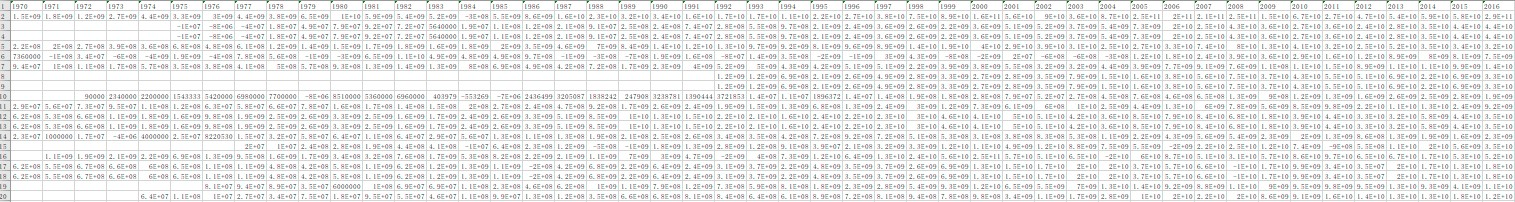
\includegraphics[width=15cm]{d.jpg}
\caption{Score}
\end{figure}
\end{appendices}
\end{document}
